\section{Introduction}

Deep neural networks excel at learning from large amounts of data, but can be poor at generalizing  learned knowledge to new datasets or environments.
Even a slight departure from a network's training domain can cause it to make spurious predictions and significantly hurt its performance~\citep{tzeng_cvpr17}.
The visual domain shift from non-photorealistic synthetic data to real images presents an even more significant challenge.
While we would like to train models on large amounts of synthetic data such as data collected from graphics game engines, such models fail to generalize to real-world imagery.
For example, a state-of-the-art semantic segmentation model trained on synthetic dashcam data fails to segment the road in real images, and its overall per-pixel label accuracy drops from 93\% (if trained on real imagery) to 54\% (if trained only on synthetic data, see Table~\ref{fig:gta-cityscapes}).


Feature-level unsupervised domain adaptation methods address this problem by aligning the features extracted from the network across the source (e.g. synthetic) and target (e.g. real) domains, without any labeled target samples.
Alignment typically involves minimizing some measure of distance between the source and target feature distributions, such as maximum mean discrepancy~\citep{long_icml15}, correlation distance~\citep{sun_taskcv16}, or adversarial discriminator accuracy ~\citep{ganin_icml15,tzeng_cvpr17}.
This class of techniques suffers from two main limitations. First, aligning marginal distributions does not enforce any semantic consistency, e.g. target features of a car may be mapped to source features of a bicycle. Second, alignment at higher levels of a deep representation can fail to model aspects of low-level appearance variance which are crucial for the end visual task. 

\begin{figure}[t]	
	\centering
	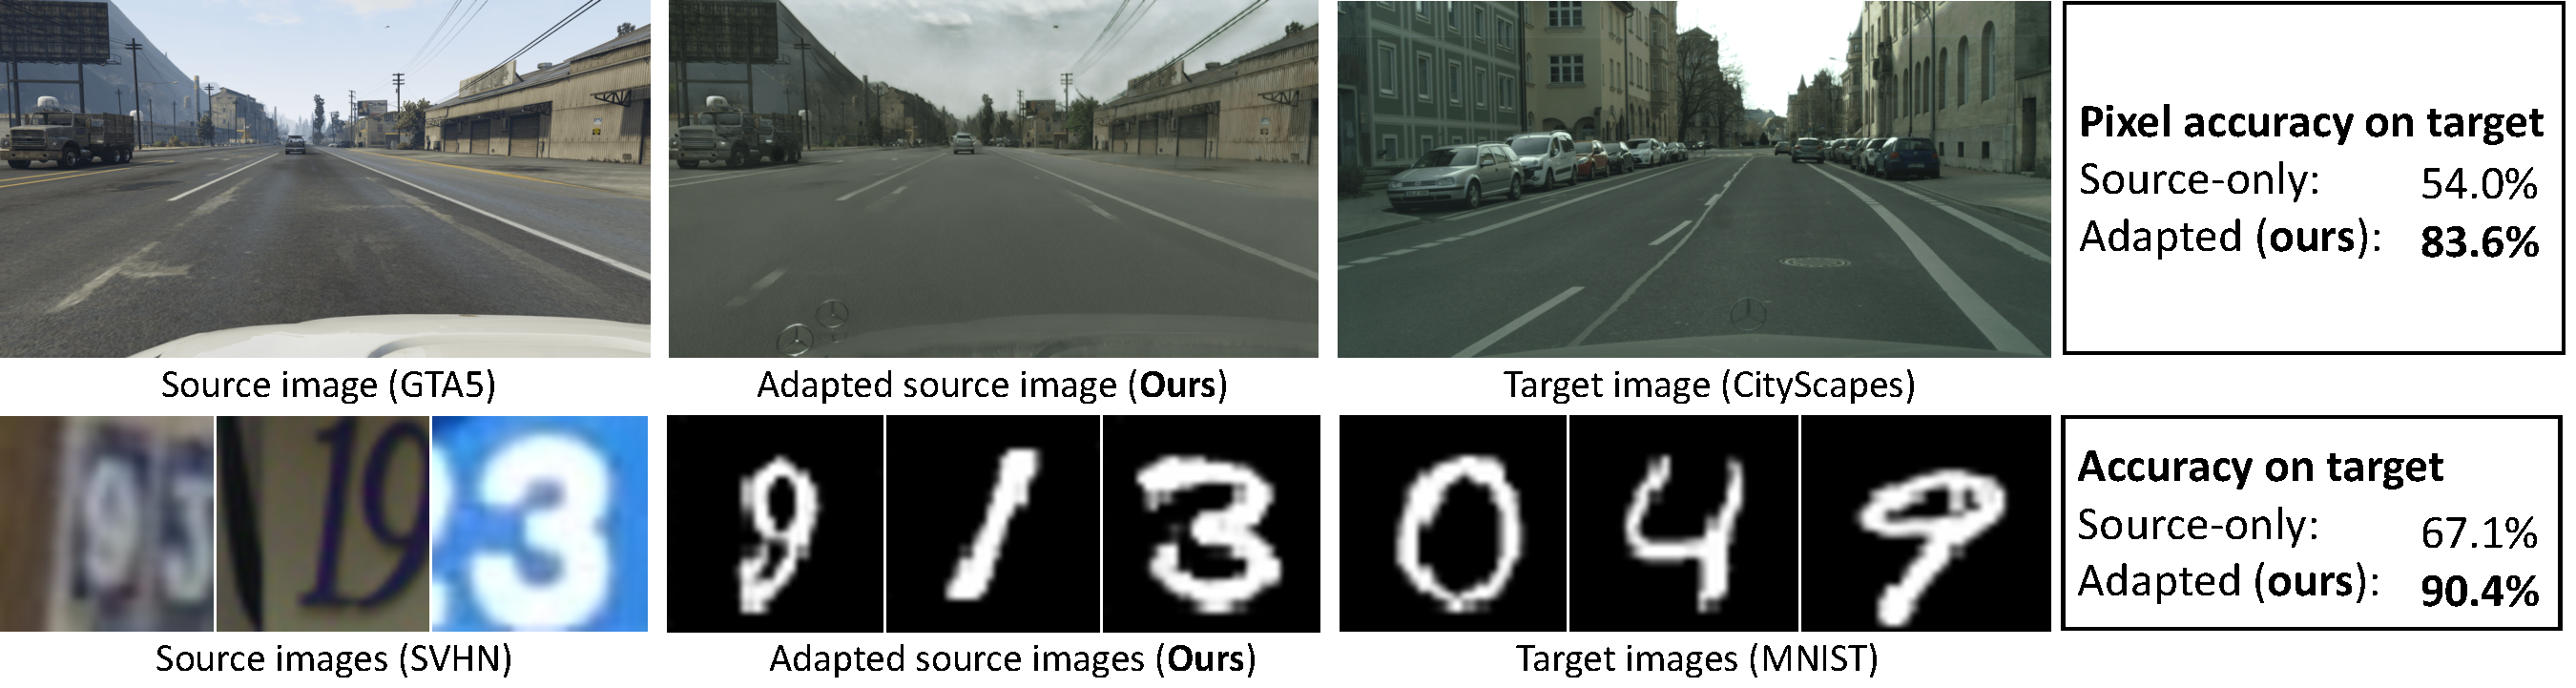
\includegraphics[width=\linewidth]{figs/cycada-fig1}
	\caption{We propose CyCADA, an adversarial unsupervised adaptation algorithm which uses cycle and semantic consistency to perform adaptation at multiple levels in a deep network. Our model provides significant performance improvements over source model baselines.}
	\label{fig:teaser}
\end{figure}

Generative pixel-level domain adaptation models perform similar distribution alignment---not in feature space but rather in raw pixel space---translating source data to the ``style'' of a target domain. Recent methods can learn to translate images given only unsupervised data from both domains~\citep{bousmalis_cvpr17,liu_arxiv16,shrivastava_cvpr17}.
The results are visually compelling, but such image-space models have only been shown to work for small image sizes and limited domain shifts. A more recent approach \citep{bousmalis_arxiv17_robotic} was applied to larger (but still not high resolution) images, but in a visually controlled image for robotic applications. 
Furthermore, they also do not necessarily preserve content: while the translated image may ``look'' like it came from the right domain, crucial semantic information may be lost. For example, a model adapting from line-drawings to photos could learn to make a line-drawing of a cat look like a photo of a dog.

How can we encourage the model to preserve semantic information in the process of distribution alignment? In this paper, we explore a simple yet powerful idea: give an additional objective to the model to reconstruct the original data from the adapted version. Cycle-consistency was recently proposed in a cross-domain image generation GAN model, CycleGAN~\citep{zhu_arxiv17}, which showed transformative image-to-image generation results, but was agnostic to any particular task.


We propose Cycle-Consistent Adversarial Domain Adaptation (CyCADA), which adapts representations at both the pixel-level and feature-level while enforcing local and global structural consistency through pixel cycle-consistency and semantic losses.
CyCADA unifies prior feature-level \citep{ganin_icml15,tzeng_cvpr17} and image-level \citep{liu_arxiv16,bousmalis_cvpr17,shrivastava_cvpr17} adversarial domain adaptation methods together with cycle-consistent image-to-image translation techniques \citep{zhu_arxiv17}, as illustrated in Table~\ref{table:compare-methods}.
It is applicable across a range of deep architectures and/or representation levels, and 
has several advantages over existing unsupervised domain adaptation methods. We use a reconstruction (cycle-consistency) loss to encourage the cross-domain transformation to preserve local structural information and a semantic loss to enforce semantic consistency. 


We apply our CyCADA model to the task of digit recognition across domains and the task of semantic segmentation of urban scenes across domains. Experiments show that our model achieves state of the art results on digit adaptation, cross-season adaptation in synthetic data, and on the challenging synthetic-to-real scenario. In the latter case, it improves per-pixel accuracy from 54\% to 82\%, nearly closing the gap to the target-trained model.

Our experiments confirm  that domain adaptation can benefit greatly from cycle-consistent pixel transformations, and that this is especially important for pixel-level semantic segmentation with contemporary FCN architectures. Further, we show that adaptation at both the pixel and representation level can offer complementary improvements with joint pixel-space and feature adaptation leading to the highest performing model for digit classification tasks. 

\begin{table}[t]
\resizebox{\textwidth}{!}{
\begin{tabular}{lcccc}
	\toprule
    & Pixel  & Feature  & Semantic  & Cycle \\
    & Loss & Loss & Loss & Consistent\\
    \midrule
    CycleGAN~\citep{zhu_arxiv17} & \checkmark & & & \checkmark\\
    Feature Adapt ~\citep{ganin_icml15,tzeng_cvpr17}& & \checkmark & \checkmark\\
    Pixel Adapt~\citep{dtn,bousmalis_cvpr17}& \checkmark & &\checkmark &  \\
%    DANN~\citep{ganin_icml15} & & \checkmark & \checkmark\\
%    ADDA~\citep{tzeng_cvpr17} & & \checkmark & \checkmark\\
%    DTN~\citep{dtn} & \checkmark & &\checkmark & \\
%    PixelDA~\citep{bousmalis_cvpr17} & \checkmark & &\checkmark & \\
    CyCADA & \checkmark & \checkmark & \checkmark & \checkmark\\
    \bottomrule
\end{tabular}
}
\caption{Our model, CyCADA, may use pixel, feature, and semantic information during adaptation while learning an invertible mapping through cycle consistency. }
\label{table:compare-methods}
\end{table}

